\addtocontents{toc}{\protect\setcounter{tocdepth}{1}}
\chapter[Diseño]{Diseño}

\section[Diseño Físico de la Base de Datos]{Diseño físico de la base de datos}

La base de datos se implementa en PostgreSQL 15, un motor relacional que se
ejecuta en un contenedor y solo es accesible desde la API a través de una red
interna. La estructura sigue la transformación del modelo conceptual descrita en
el capítulo anterior: cada cuidador es la raíz de sus datos y las tablas que
dependen de él llevan una clave foránea con eliminación en cascada
(\texttt{ON DELETE CASCADE}), de modo que al borrar la cuenta se eliminan sus
pacientes, registros, recordatorios, conversaciones, favoritos y claves. El
Listado~\ref{lst:esquema-sql} resume el esquema y el Anexo~E describe cada
columna. Las columnas jsonb llamadas cifrados contienen únicamente texto cifrado
con AES-256-GCM en el teléfono del cuidador, y el servidor no dispone de la clave
para descifrarlas.

\begin{lstlisting}[language={},basicstyle=\ttfamily\fontsize{7.2pt}{8.6pt}\selectfont,columns=fullflexible,breaklines=true,caption={Esquema relacional resumido de OnCuidar (PostgreSQL 15).},label={lst:esquema-sql}]
CREATE TABLE usuarios (            -- cuidador
  id uuid PRIMARY KEY DEFAULT gen_random_uuid(),
  correo text UNIQUE NOT NULL,
  contrasena_hash text,            -- bcrypt
  correo_verificado boolean DEFAULT false,
  correo_respaldo_hash text,       -- solo HMAC del correo de respaldo
  cifrados jsonb DEFAULT '{}',     -- nombre, telefono, parentesco (cifrados)
  creado_en timestamptz DEFAULT now() );   -- y columnas de correos pendientes

CREATE TABLE pacientes (
  usuario_id uuid REFERENCES usuarios(id) ON DELETE CASCADE,
  id text,
  notificaciones_activas boolean, maximo_registros_dia int, archivado boolean,
  cifrados jsonb,                  -- nombre, RUT, edad, diagnostico, centro, contacto
  PRIMARY KEY (usuario_id, id) );

CREATE TABLE registros_clinicos (
  usuario_id uuid, paciente_id text, id text,
  fecha timestamptz, tipo_registro text, nivel_alerta text,   -- en claro
  cifrados jsonb,                  -- signos vitales, sintomas, observaciones
  PRIMARY KEY (usuario_id, paciente_id, id),
  FOREIGN KEY (usuario_id, paciente_id) REFERENCES pacientes
    ON DELETE CASCADE );           -- indices por (usuario, paciente, fecha/creado_en)

CREATE TABLE recordatorios (
  usuario_id uuid, paciente_id text, id text, activo boolean,
  cifrados jsonb,                  -- titulo, descripcion, programacion
  PRIMARY KEY (usuario_id, paciente_id, id),
  FOREIGN KEY (usuario_id, paciente_id) REFERENCES pacientes
    ON DELETE CASCADE );

CREATE TABLE conversaciones (
  usuario_id uuid REFERENCES usuarios(id) ON DELETE CASCADE,
  id text, ultima_actividad timestamptz,
  cifrados jsonb,                  -- titulo y mensajes
  PRIMARY KEY (usuario_id, id) );

CREATE TABLE material_educativo ( -- catalogo compartido, de solo lectura
  id text PRIMARY KEY, titulo text, categoria text, tema text, cuerpo text,
  url_imagen text, url_archivo text, url_miniatura text,
  tipo_archivo text, tamano_bytes bigint );

CREATE TABLE favoritos (          -- tabla puente N:M
  usuario_id uuid REFERENCES usuarios(id) ON DELETE CASCADE,
  material_id text,
  PRIMARY KEY (usuario_id, material_id) );

CREATE TABLE claves_datos (       -- clave de datos sellada con la clave maestra
  usuario_id uuid PRIMARY KEY REFERENCES usuarios(id) ON DELETE CASCADE,
  clave_sellada text NOT NULL );

CREATE TABLE tokens_restablecer ( -- enlaces de un solo uso (1 h), solo hash
  token_hash text PRIMARY KEY, usuario_id uuid REFERENCES usuarios(id)
    ON DELETE CASCADE, expira_en timestamptz, usado boolean );
-- tokens_correo (verificacion y cambio de correos) y esperas_recuperacion
-- (limite de reenvios) siguen el mismo patron.
\end{lstlisting}

El motor admite funciones y disparadores, pero el diseño concentra las reglas de
integridad en las claves y en la API, que aplican las siguientes restricciones.

\begin{itemize}
    \item \emph{Integridad referencial}: las claves foráneas, simples o
    compuestas, impiden crear un registro clínico o un recordatorio sin su
    paciente, y la eliminación en cascada evita datos huérfanos.
    \item \emph{Índices}: los registros clínicos y los recordatorios tienen un
    índice por usuario, paciente y fecha de creación, y las conversaciones por
    usuario y última actividad, que son los órdenes con que la aplicación
    lista los datos.
    \item \emph{Autorización por usuario}: cada petición lleva un token JWT y
    toda consulta se filtra por el usuario del token. Un recurso de otro
    usuario responde como inexistente.
    \item \emph{Datos sensibles cifrados}: la API rechaza con error 400 cualquier
    escritura que incluya un campo clínico en claro, y solo acepta en la columna
    cifrados claves que corresponden a texto cifrado.
    \item \emph{Contenido educativo}: la tabla material\_educativo es de solo
    lectura para la aplicación. La API la carga al iniciar si está vacía.
    \item \emph{Clave de datos}: la ruta \texttt{POST /clave-datos} crea la clave
    de cifrado del usuario la primera vez y la sella con AES-256-GCM usando una
    clave maestra definida en el entorno del servidor. La tabla claves\_datos
    solo guarda la clave sellada, y el cliente nunca accede a ella directamente.
    \item \emph{Credenciales y enlaces}: las contraseñas se guardan con bcrypt y
    los enlaces de correo, que son de un solo uso y vencen en una hora, solo
    registran el hash de su token. El correo de respaldo se conserva únicamente
    como HMAC.
\end{itemize}

\section[Diseño de Arquitectura Funcional]{Diseño de arquitectura funcional}

La Figura~\ref{fig:arquitectura} descompone el sistema en siete módulos
funcionales. Sus funciones corresponden a los casos de uso del capítulo
anterior.

\begin{figure}[H]
    \centering
    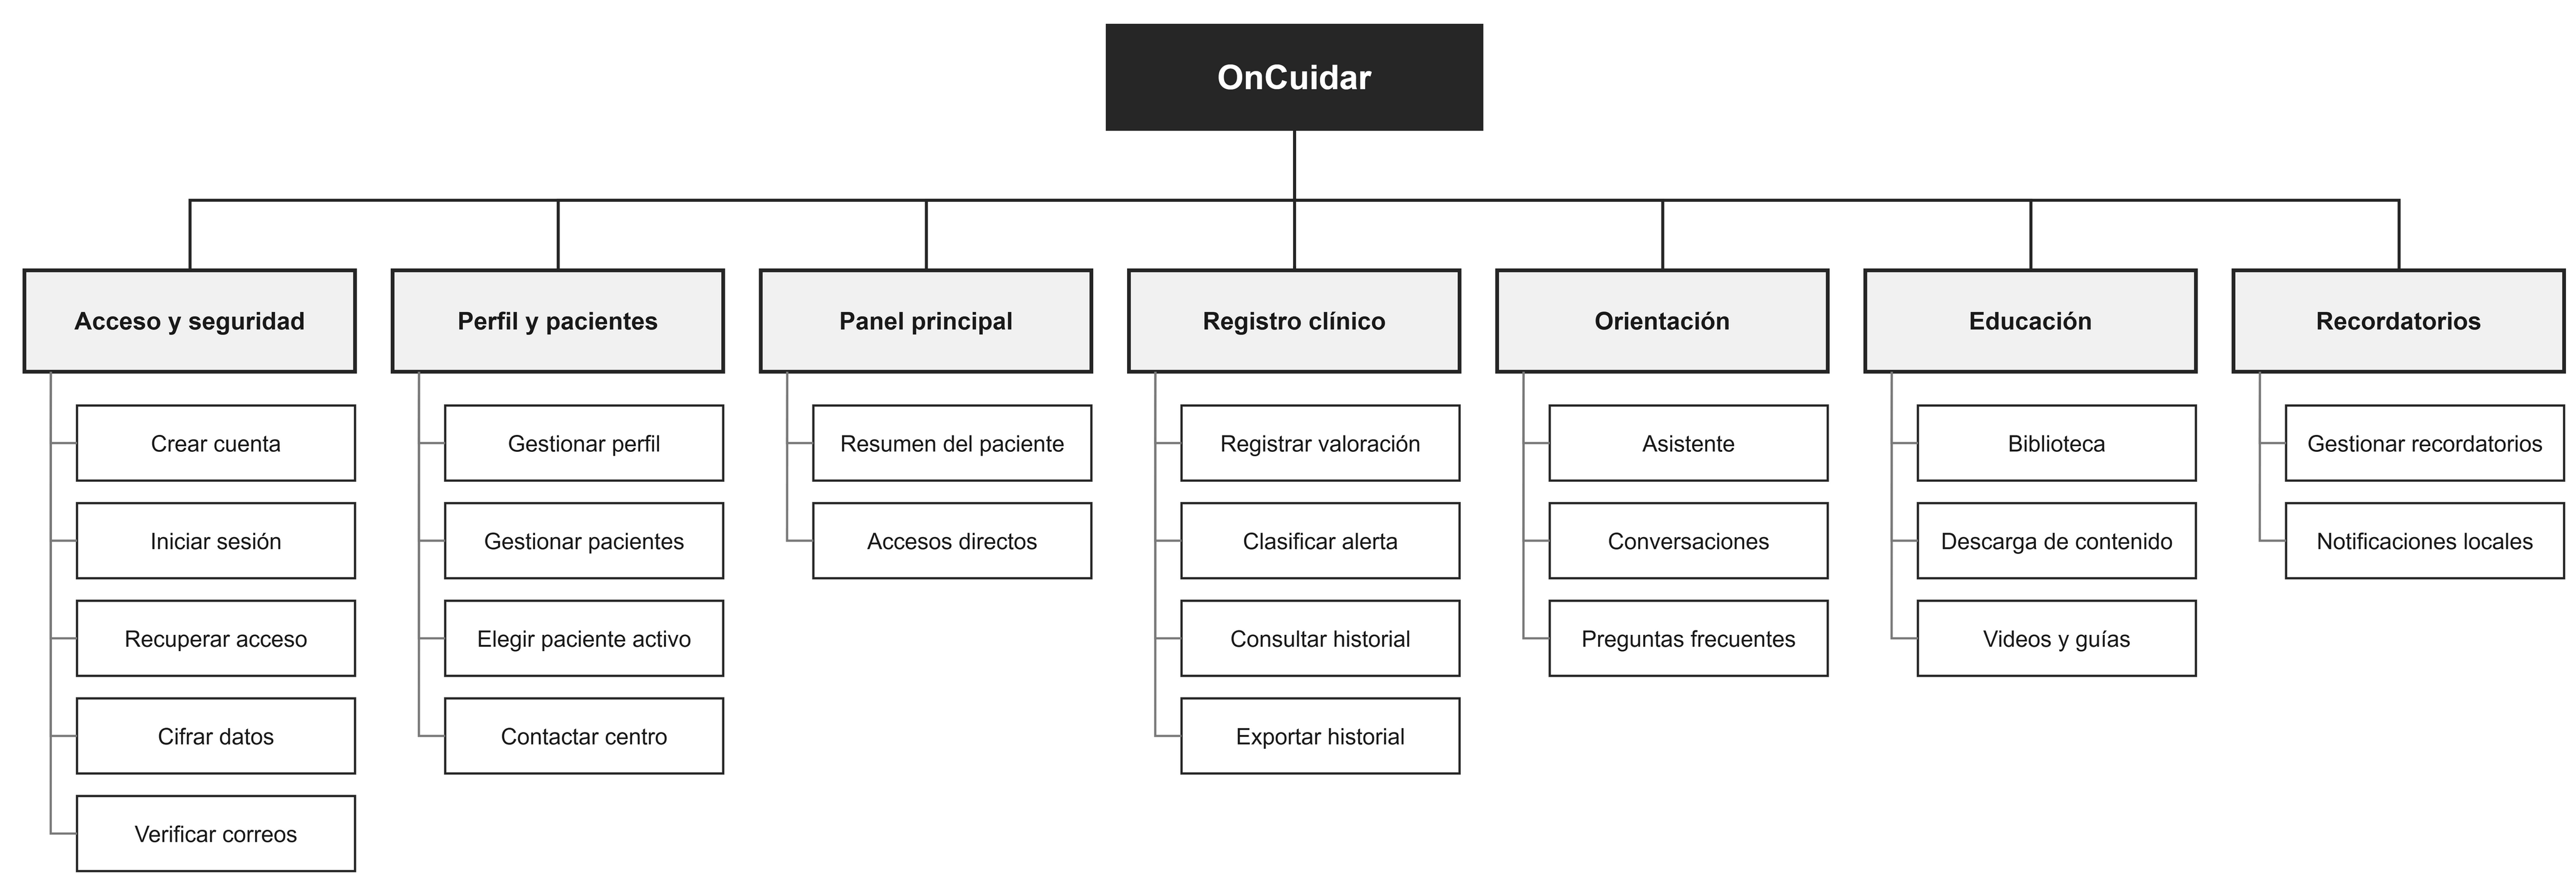
\includegraphics[width=\textwidth]{figures/diseno/arquitectura.png}
    \caption{Árbol de descomposición funcional de OnCuidar.}
    \label{fig:arquitectura}
\end{figure}

Internamente, el código se organiza por funcionalidad y, dentro de cada una,
en tres capas, siguiendo la guía de arquitectura de aplicaciones de Flutter. Cada
funcionalidad (autenticación, pacientes, registro clínico, historial, panel
principal, chat, preguntas frecuentes, recordatorios, biblioteca y perfil) tiene
una carpeta de dominio, con los modelos y las reglas puras, como el motor de
reglas clínicas; una de datos, con el repositorio que guarda y lee en la API del
servidor cifrando y descifrando los campos sensibles; y una de presentación, con las
pantallas, sus widgets y un controlador que reúne la lógica de cada pantalla. El
estado se expone a las pantallas con Riverpod y se actualiza mediante consultas
periódicas a la API, en lugar de suscripciones en tiempo real.

Los repositorios comparten una base de datos segura común, que concentra el
cifrado, la cola de escrituras sin conexión y la identidad del cuidador, pero no
dependen entre sí. Cuando una acción involucra a más de un área, la coordina un
caso de uso: por ejemplo, archivar o eliminar un paciente también cancela los
avisos de sus recordatorios. Los servicios transversales (cifrado,
conectividad, notificaciones y sincronización) forman un núcleo común, y los
componentes visuales reutilizados por varias pantallas, una carpeta compartida.
Esta separación permite probar cada capa de forma aislada y modificar una
pantalla sin tocar la lógica de datos.

Al iniciar sesión, una compuerta de datos restaura la clave de cifrado del
usuario o la solicita al servidor antes de mostrar cualquier información del
paciente. Luego se descarga en segundo plano el contenido educativo para dejarlo
disponible sin conexión.

\section[Diseño de Arquitectura Física y Despliegue]{Diseño de arquitectura física y despliegue}

La Figura~\ref{fig:despliegue} muestra la arquitectura física. El cuidador
usa la aplicación Flutter en un teléfono Android, que cifra los datos sensibles
con AES-GCM antes de enviarlos y guarda en un almacenamiento seguro el token de
sesión y la clave de datos. La aplicación se comunica con la API mediante
HTTP y JSON, con el token JWT en cada petición; si no hay conexión, la cola de
escrituras conserva las operaciones y las envía al recuperar la red.

\begin{figure}[H]
    \centering
    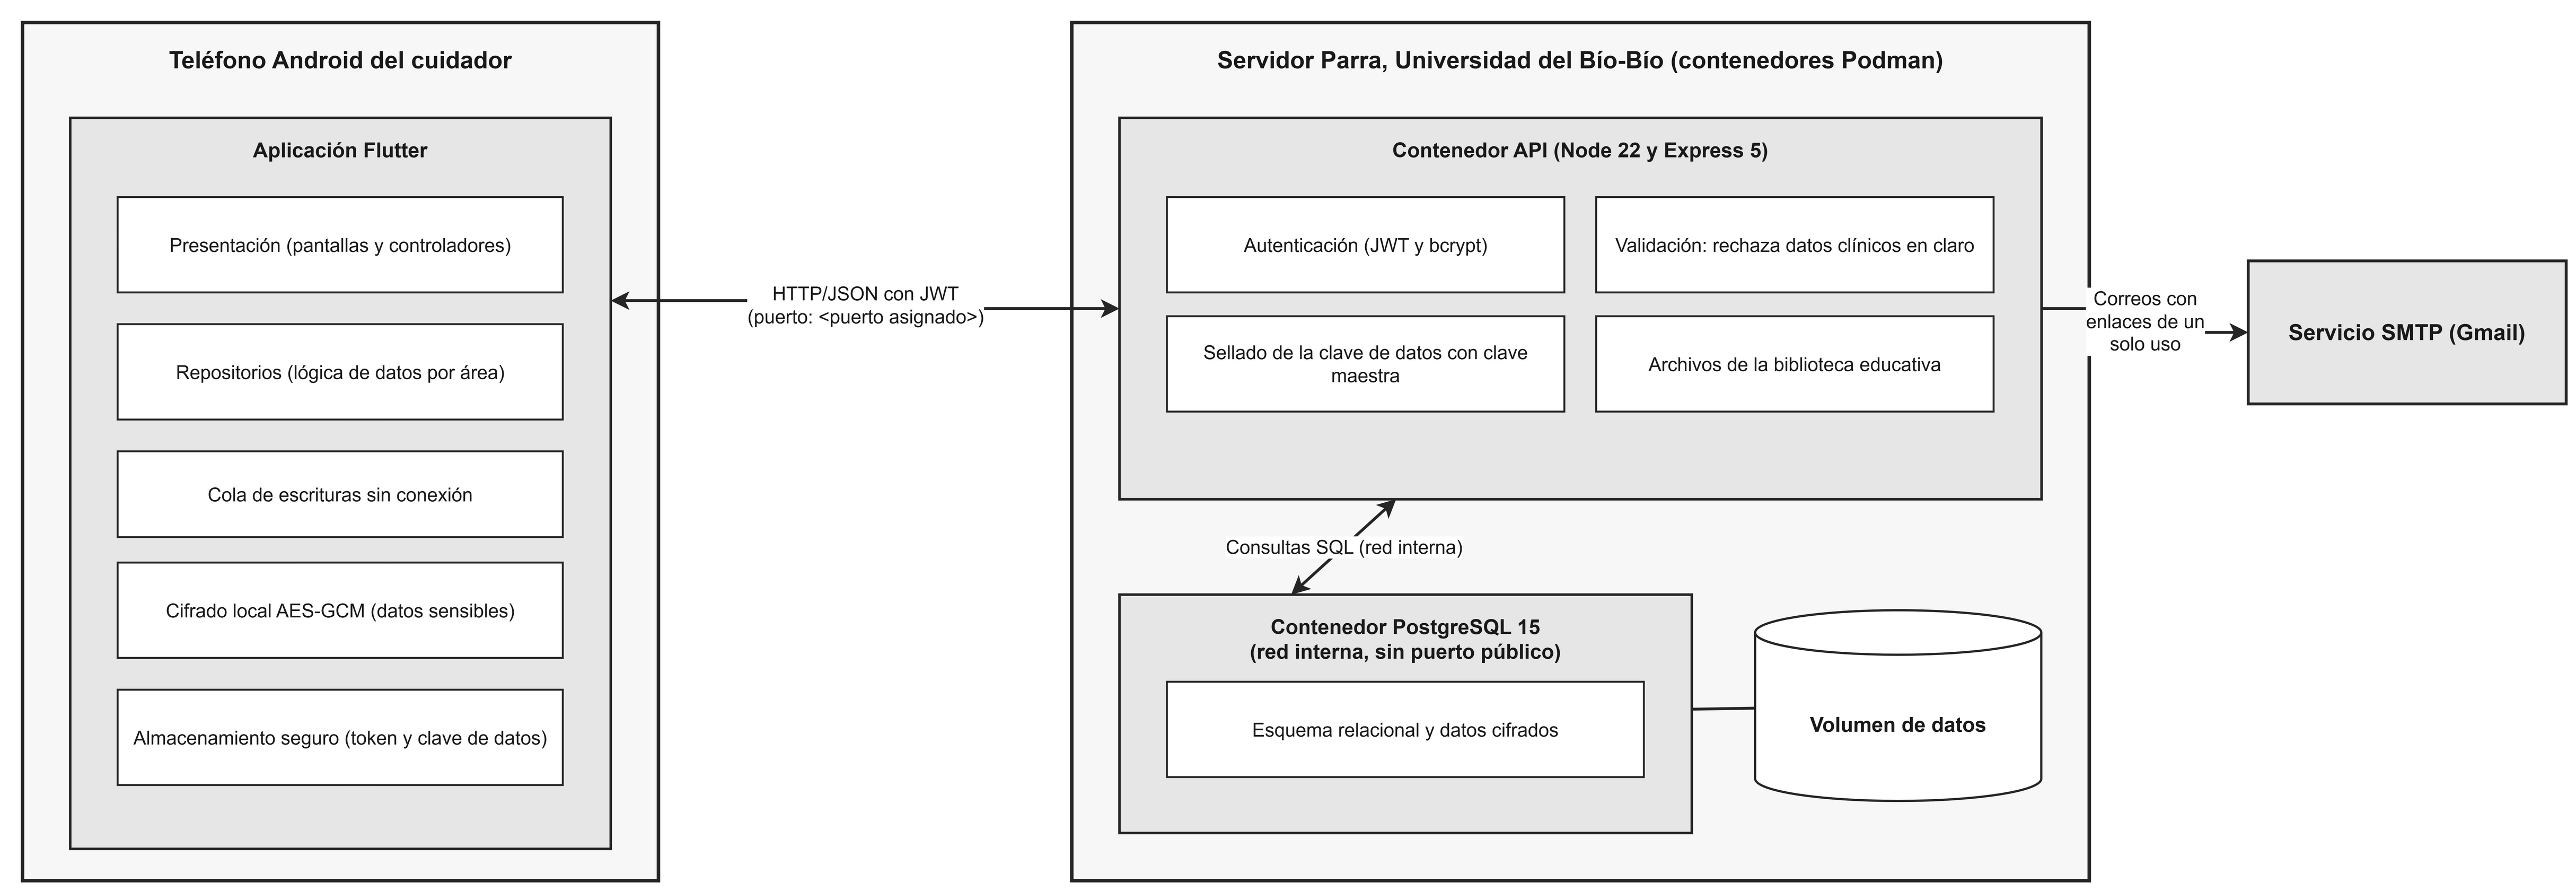
\includegraphics[width=\textwidth]{figures/diseno/despliegue.png}
    \caption{Arquitectura física y despliegue de OnCuidar.}
    \label{fig:despliegue}
\end{figure}

El servidor ejecuta dos contenedores definidos en Docker Compose y destinados a
Podman en el servidor Parra de la Universidad del Bío-Bío. El contenedor de la API
(Node 22 y Express 5) es el único que publica un puerto y también sirve los
archivos de la biblioteca educativa. El contenedor de PostgreSQL permanece en la
red interna, sin puerto público, y guarda sus datos en un volumen persistente. Para
enviar los correos de verificación y recuperación, la API utiliza un servicio
SMTP externo (Gmail). El sistema funciona en un entorno local; su despliegue en
el servidor de la universidad queda pendiente de la activación de la cuenta y de
la entrega de los puertos definitivos. La Tabla~\ref{tab:puertos} resume los
servicios.

\begin{table}[H]
\centering
\small
\tablazebra
\caption{Servicios del despliegue y su exposición.}
\label{tab:puertos}
\begin{tabularx}{\textwidth}{P{0.80}P{0.90}P{0.70}P{0.60}}
\toprule
\filaencabezado \encab{Servicio} & \encab{Función} & \encab{Puerto} & \encab{Acceso} \\
\midrule
API (Node y Express) & Autenticación, validación y acceso a datos & \textless puerto asignado\textgreater{} (3000 en el contenedor) & Público, con JWT \\
PostgreSQL 15 & Almacenamiento relacional de los datos cifrados & 5432 solo en la red interna & Solo la API \\
Servicio SMTP (Gmail) & Entrega de correos con enlaces de un solo uso & Definido por el proveedor & Salida desde la API \\
\bottomrule
\end{tabularx}
\end{table}

\section[Diseño de Interfaz y Navegación]{Diseño de interfaz y navegación}

\subsection*{Estándar de pantalla}

Todas las pantallas siguen el mismo esquema.

\begin{itemize}
    \item \emph{Encabezado}: cabecera con degradado dorado, título de la
    pantalla y, en el panel principal, saludo y nombre del paciente activo.
    \item \emph{Logo}: la marca OnCuidar aparece en la carga inicial, la
    bienvenida y el pie del perfil.
    \item \emph{Ingreso de datos}: campos con etiqueta visible, validación en
    línea y mensajes de error bajo el campo afectado.
    \item \emph{Botones de opción general}: acción principal destacada en
    dorado (guardar, crear, continuar) y acción secundaria con contorno
    (cancelar, volver).
    \item \emph{Botones específicos}: acciones propias de cada pantalla, como
    exportar en el historial o marcar como favorito en la biblioteca.
    \item \emph{Menú}: barra inferior permanente con Inicio, Chat, Registro,
    Aprende y Perfil.
    \item \emph{Estados de alerta}: verde, amarillo y rojo, siempre acompañados
    de un ícono y un texto.
\end{itemize}

\subsection*{Mapa de navegación}

La Figura~\ref{fig:navegacion} muestra las rutas de la aplicación. Si existe una
sesión activa, la carga inicial lleva directamente al panel principal. En caso
contrario, pasa por la bienvenida, desde donde el cuidador inicia sesión o crea
su cuenta. Una vez dentro, la barra inferior da acceso a los cinco módulos
principales y el panel principal ofrece accesos directos al historial y a los
recordatorios.

\begin{figure}[H]
    \centering
    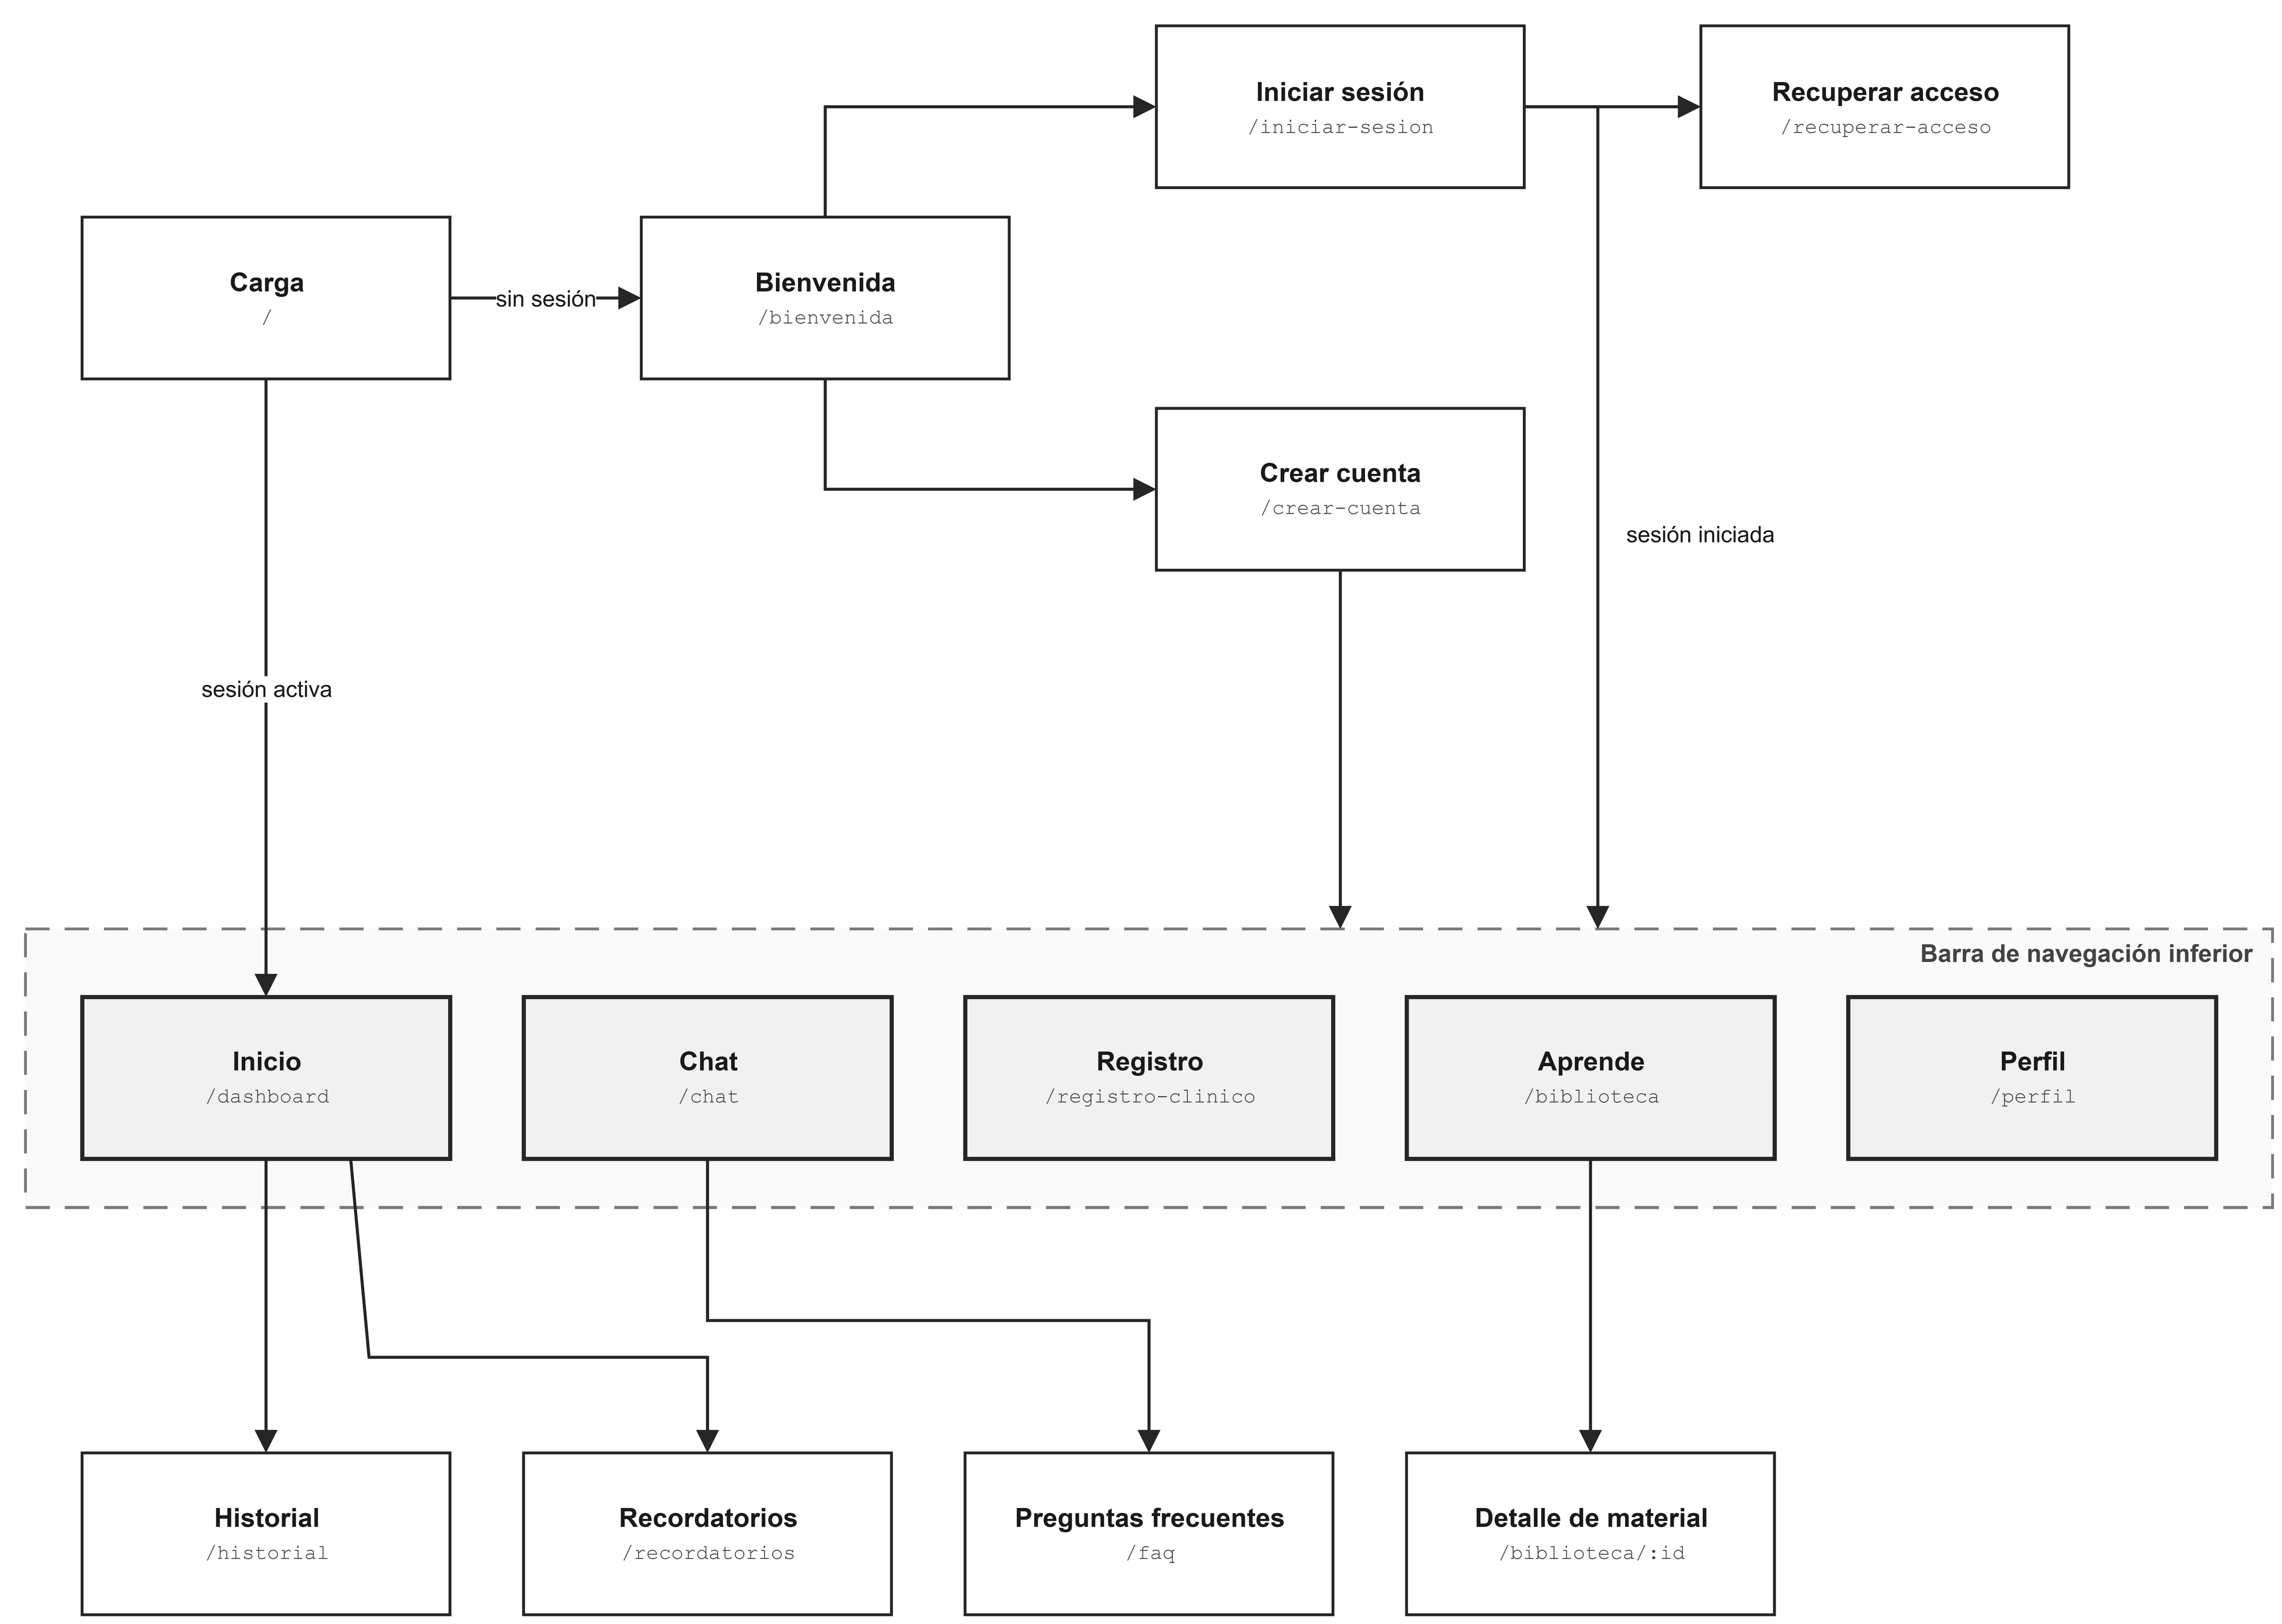
\includegraphics[width=0.95\textwidth]{figures/diseno/navegacion.png}
    \caption{Mapa de navegación de OnCuidar.}
    \label{fig:navegacion}
\end{figure}

\subsection*{Prototipos de interfaz}

Los prototipos se diseñaron en Figma y se revisaron con la contraparte antes de
construir cada módulo. La paleta cálida, inspirada en el lazo dorado del cáncer
infantil, busca transmitir cercanía y reducir la fatiga visual. Las figuras
siguientes presentan el acceso, el seguimiento, el apoyo educativo y la gestión.

\begin{figure}[H]
    \centering
    \begin{subfigure}[b]{0.30\textwidth}
        \centering
        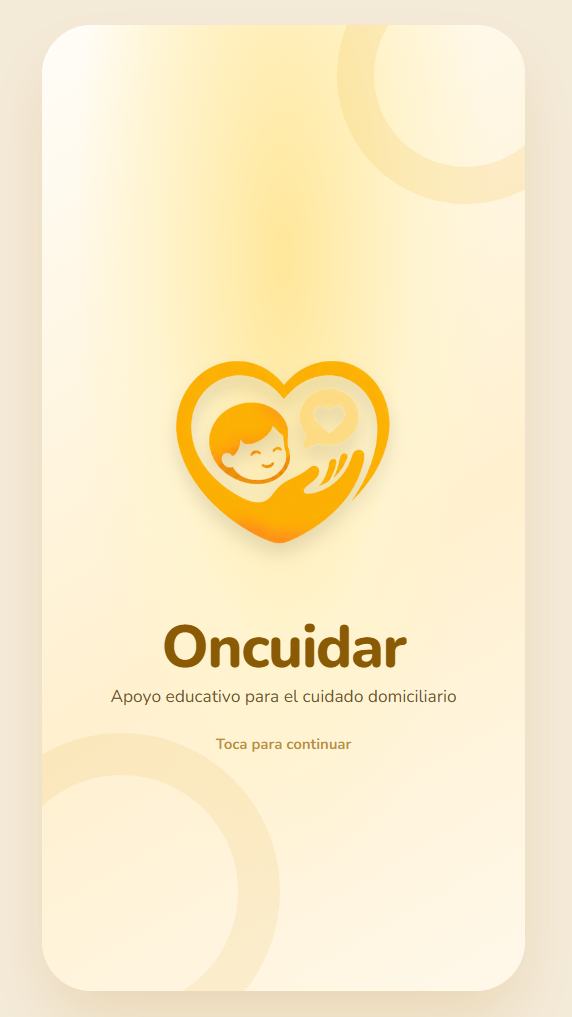
\includegraphics[width=\linewidth]{figures/mockups/01_splash.png}
        \caption{Pantalla de inicio}
        \label{fig:mockup-splash}
    \end{subfigure}
    \hfill
    \begin{subfigure}[b]{0.30\textwidth}
        \centering
        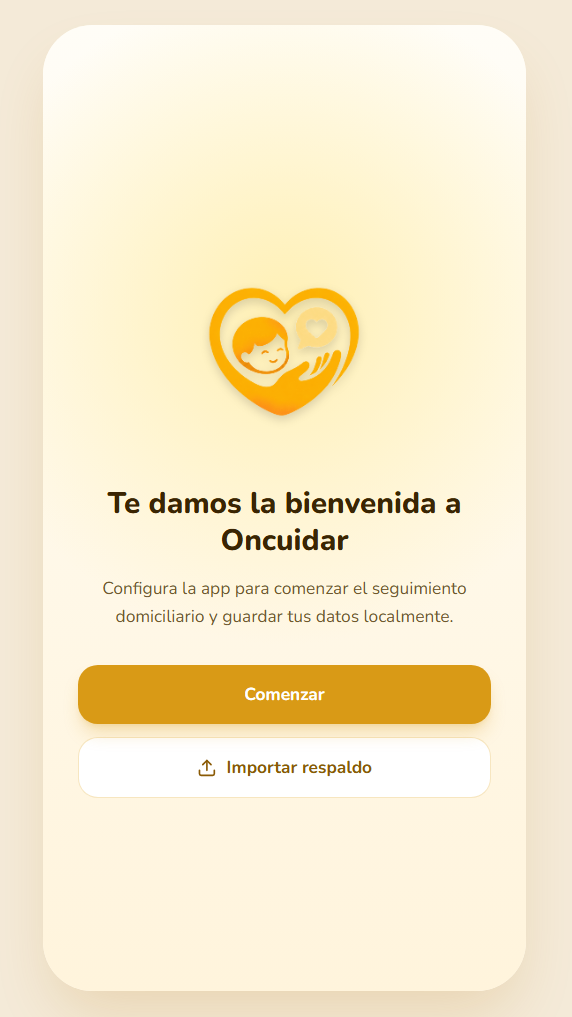
\includegraphics[width=\linewidth]{figures/mockups/02_bienvenida.png}
        \caption{Bienvenida}
        \label{fig:mockup-bienvenida}
    \end{subfigure}
    \hfill
    \begin{subfigure}[b]{0.30\textwidth}
        \centering
        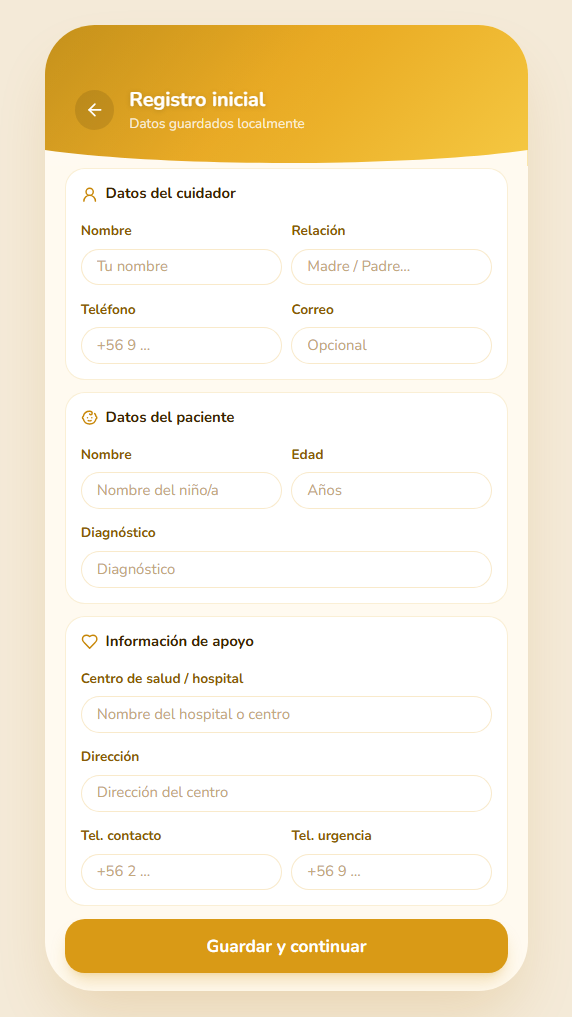
\includegraphics[width=\linewidth]{figures/mockups/03_registro_inicial.png}
        \caption{Registro inicial}
        \label{fig:mockup-registro-inicial}
    \end{subfigure}
    \caption{Flujo de \textit{onboarding}: acceso al sistema y configuración del perfil.}
    \label{fig:mockups-flujo-inicial}
\end{figure}

\begin{figure}[H]
    \centering
    \begin{subfigure}[b]{0.30\textwidth}
        \centering
        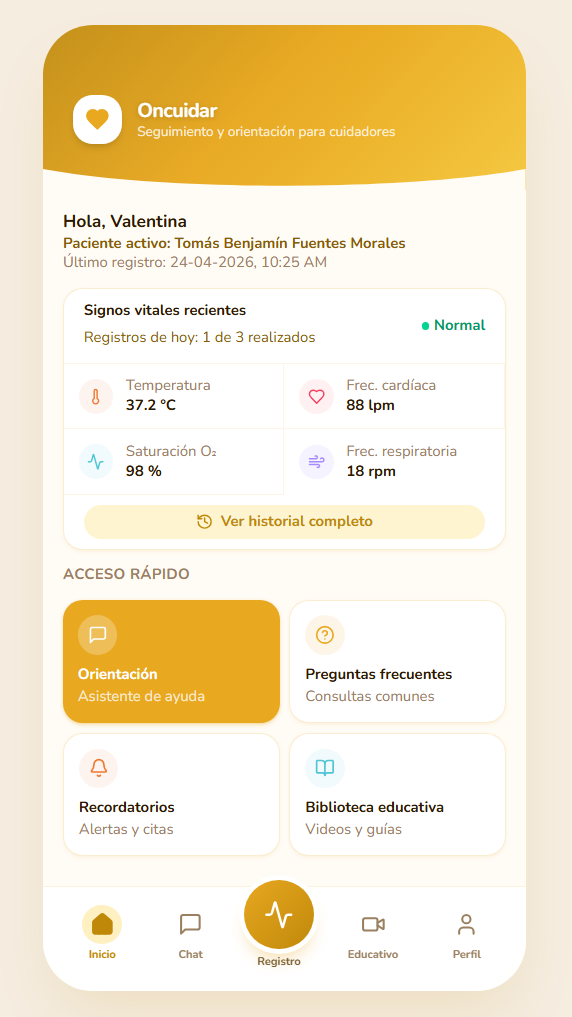
\includegraphics[width=\linewidth]{figures/mockups/04_inicio.png}
        \caption{Inicio (\textit{Dashboard})}
        \label{fig:mockup-inicio}
    \end{subfigure}
    \hfill
    \begin{subfigure}[b]{0.30\textwidth}
        \centering
        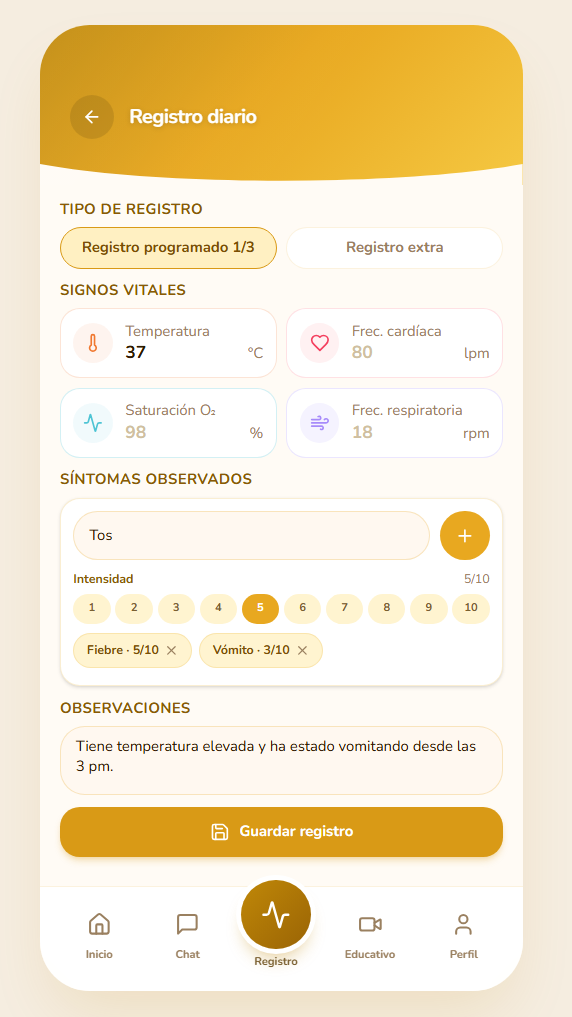
\includegraphics[width=\linewidth]{figures/mockups/05_registro_diario.png}
        \caption{Registro diario}
        \label{fig:mockup-registro-diario}
    \end{subfigure}
    \hfill
    \begin{subfigure}[b]{0.30\textwidth}
        \centering
        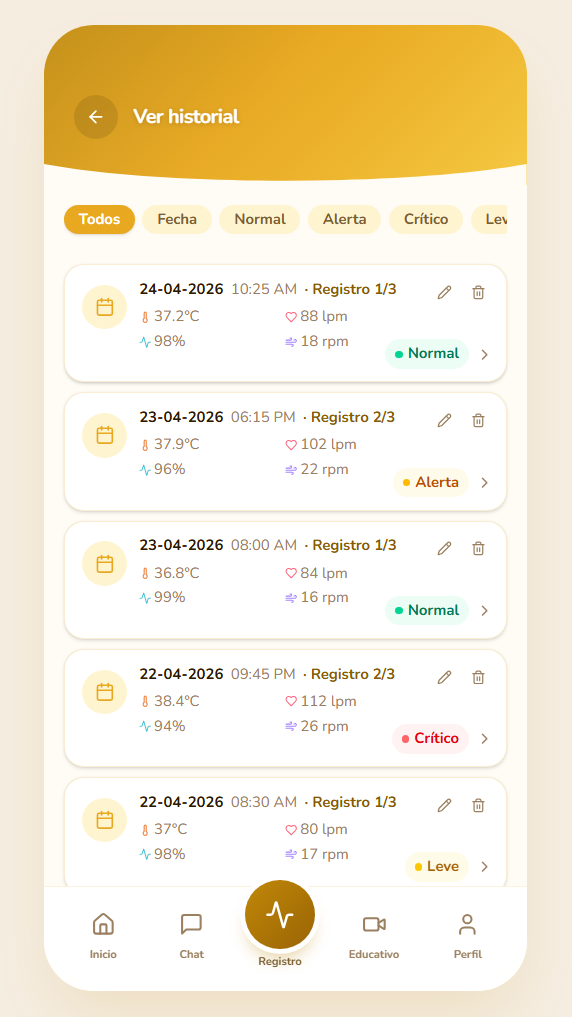
\includegraphics[width=\linewidth]{figures/mockups/06_historial.png}
        \caption{Historial clínico}
        \label{fig:mockup-historial}
    \end{subfigure}
    \caption{Módulo de bitácora: visualización del estado, ingreso de métricas y consulta cronológica.}
    \label{fig:mockups-seguimiento}
\end{figure}

\begin{figure}[H]
    \centering
    \begin{subfigure}[b]{0.30\textwidth}
        \centering
        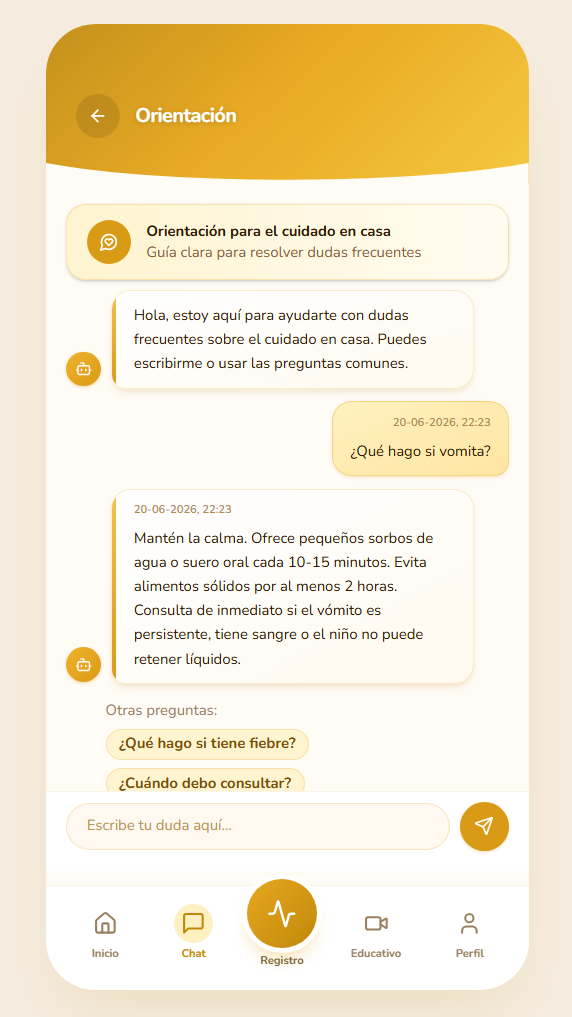
\includegraphics[width=\linewidth]{figures/mockups/07_orientacion.png}
        \caption{Orientación guiada}
        \label{fig:mockup-orientacion}
    \end{subfigure}
    \hfill
    \begin{subfigure}[b]{0.30\textwidth}
        \centering
        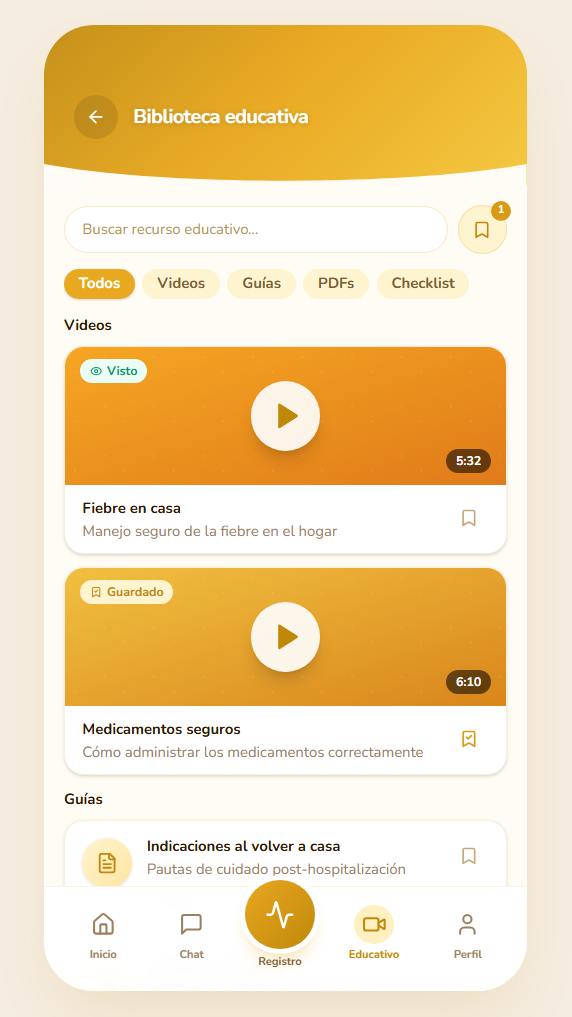
\includegraphics[width=\linewidth]{figures/mockups/08_biblioteca.png}
        \caption{Biblioteca de salud}
        \label{fig:mockup-biblioteca}
    \end{subfigure}
    \hfill
    \begin{subfigure}[b]{0.30\textwidth}
        \centering
        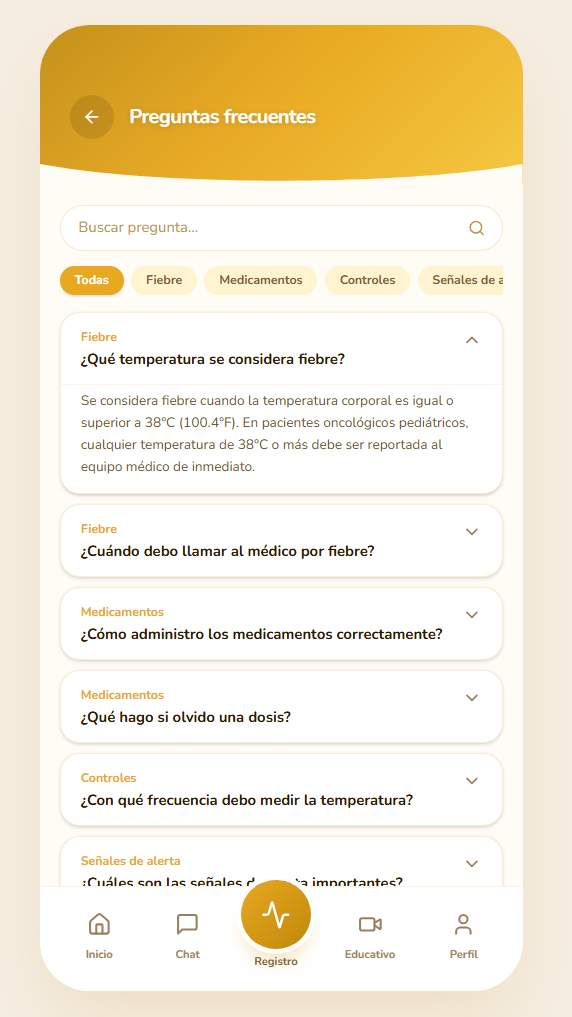
\includegraphics[width=\linewidth]{figures/mockups/09_preguntas_frecuentes.png}
        \caption{Preguntas frecuentes}
        \label{fig:mockup-preguntas}
    \end{subfigure}
    \caption{Módulo de apoyo: asistente de reglas, repositorio de lectura y resolución de dudas.}
    \label{fig:mockups-apoyo-educativo}
\end{figure}

\begin{figure}[H]
    \centering
    \begin{subfigure}[b]{0.30\textwidth}
        \centering
        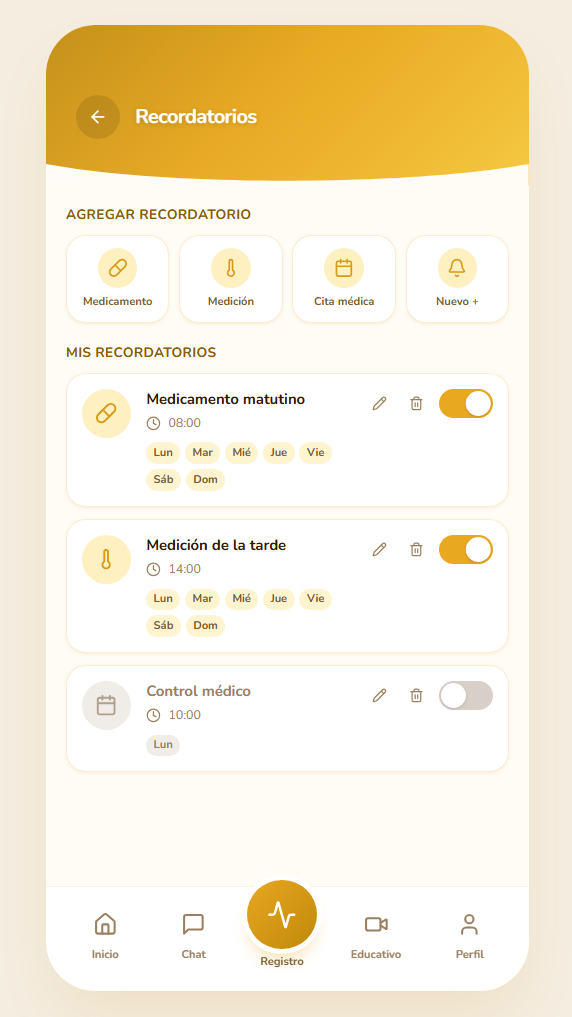
\includegraphics[width=\linewidth]{figures/mockups/10_recordatorios.png}
        \caption{Gestión de alarmas}
        \label{fig:mockup-recordatorios}
    \end{subfigure}
    \hfill
    \begin{subfigure}[b]{0.30\textwidth}
        \centering
        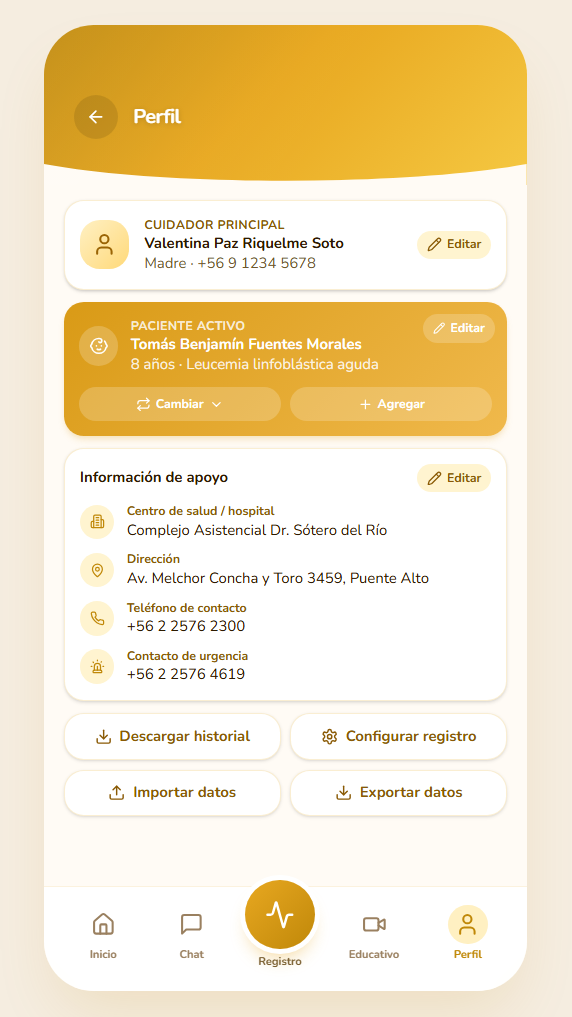
\includegraphics[width=\linewidth]{figures/mockups/11_perfil.png}
        \caption{Perfil y exportación de informes}
        \label{fig:mockup-perfil}
    \end{subfigure}
    \caption{Módulo de gestión: configuración de notificaciones y administración de datos.}
    \label{fig:mockups-gestion}
\end{figure}

\section[Especificación de Módulos]{Especificación de módulos}

La Tabla~\ref{tab:modulos} especifica los módulos de programa principales, con
sus parámetros de entrada y de salida.

\begingroup
\small
\tablazebra
\begin{xltabular}{\textwidth}{P{0.35}P{1.05}P{1.40}P{1.20}}
    \caption{Especificación de los módulos de programa.}
    \label{tab:modulos}\\
    \toprule
    \filaencabezado \encab{N°} & \encab{Módulo} & \encab{Parámetros de entrada} & \encab{Parámetros de salida} \\
    \midrule
    \endfirsthead
    \rowcolor{white}\multicolumn{4}{@{}l}{\footnotesize\itshape Tabla \thetable{} (continuación)} \\
    \toprule
    \filaencabezado \encab{N°} & \encab{Módulo} & \encab{Parámetros de entrada} & \encab{Parámetros de salida} \\
    \midrule
    \endhead
    \midrule
    \rowcolor{white}\multicolumn{4}{r@{}}{\footnotesize\itshape Continúa en la página siguiente} \\
    \endfoot
    \bottomrule
    \endlastfoot
    M01 & Registrar cuenta\newline{\scriptsize servicio\_alta\_cuenta} &
    datos: DatosRegistro (cuidador, paciente, centro, contacto,
    correo y contraseña) & ResultadoRegistro (éxito o mensaje de error) \\
    M02 & Cifrar dato\newline{\scriptsize servicio\_cifrado} &
    uid: String, texto: String & String con el texto cifrado \\
    M03 & Descifrar dato\newline{\scriptsize servicio\_cifrado} &
    uid: String, valor: String & String con el texto original \\
    M04 & Evaluar alerta\newline{\scriptsize motor\_reglas\_clinicas} &
    signos: SignosVitales, sintomas: List<EntradaSintoma> &
    EvaluacionAlerta (nivel y mensajes) \\
    M05 & Guardar registro clínico\newline{\scriptsize repositorio\_registros\_clinicos} &
    idPaciente: String, registro: RegistroClinico &
    Sin retorno. Lanza un error si el registro no pertenece al paciente. \\
    M06 & Leer historial\newline{\scriptsize repositorio\_registros\_clinicos} &
    idPaciente: String & Stream<List<RegistroClinico>> con los 50 más
    recientes \\
    M07 & Generar informe PDF\newline{\scriptsize exportador\_pdf} &
    registros, paciente, nombreCuidador,
    fechaInicio, fechaFin, generadoEn &
    Uint8List con el documento PDF \\
    M08 & Generar planilla Excel\newline{\scriptsize exportador\_excel} &
    Los mismos parámetros de M07 & Uint8List con el archivo XLSX \\
    M09 & Programar notificación\newline{\scriptsize servicio\_notificaciones} &
    id: int, titulo, cuerpo: String,
    fechaHora: DateTime, diasRepeticion, mensual &
    Sin retorno. Deja la notificación agendada en el dispositivo. \\
    M10 & Descargar material\newline{\scriptsize servicio\_cache\_contenido} &
    url: String & File con la copia local del material \\
\end{xltabular}
\endgroup

Los módulos provenientes de librerías externas se describen en la
Tabla~\ref{tab:librerias}.

\begin{table}[H]
\centering
\small
\tablazebra
\caption{Módulos utilizados desde librerías externas.}
\label{tab:librerias}
\begin{tabularx}{\textwidth}{P{0.85}P{1.05}P{1.10}}
\toprule
\filaencabezado \encab{Nombre} & \encab{Objetivo} & \encab{Parámetros principales} \\
\midrule
AesGcm.with256bits (cryptography) & Cifrar y descifrar datos
sensibles & Clave secreta, texto y nonce \\
zonedSchedule (flutter\_local\_notifications) & Agendar una
notificación local & Identificador, título, cuerpo y fecha con zona horaria \\
Document (pdf) & Construir el informe PDF & Páginas y widgets de
contenido \\
Excel.createExcel (excel) & Construir la planilla XLSX & Hojas, filas
y estilos de celda \\
VideoPlayerController (video\_player) & Reproducir videos educativos &
Archivo local o URL del video \\
launchUrl (url\_launcher) & Abrir llamadas y mapas & URI tel:
o URL de Google Maps \\
\bottomrule
\end{tabularx}
\end{table}

\addtocontents{toc}{\protect\setcounter{tocdepth}{2}}
